% Exact example 2, same x/y scale.
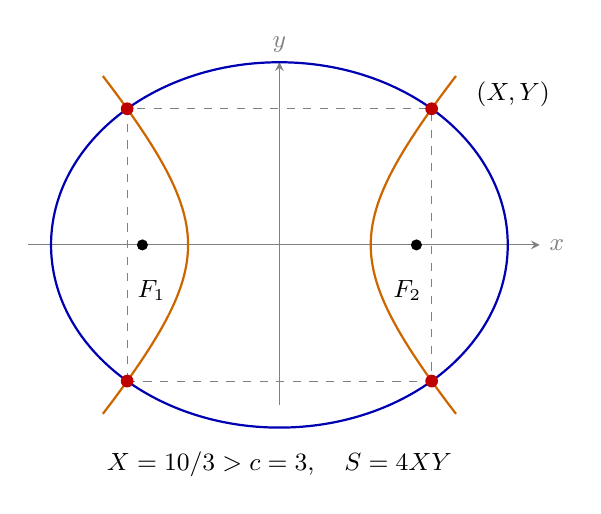
\begin{tikzpicture}[x=.58cm,y=.58cm,>=stealth,font=\small]
\draw[->,gray] (-5.5,0)--(5.7,0) node[right] {$x$};
\draw[->,gray] (0,-3.5)--(0,4) node[above] {$y$};
\draw[blue!70!black,thick] (0,0) ellipse (5 and 4);
\foreach \s in {-1,1} {
\draw[orange!80!black,thick,domain=-3.7:3.7,samples=100,variable=\t]
 plot ({\s*2*sqrt(1+\t*\t/5)},\t);}
\draw[gray,dashed] (-10/3,{-4*sqrt(5)/3}) rectangle (10/3,{4*sqrt(5)/3});
\foreach \s in {-1,1} {\foreach \t in {-1,1}
 {\fill[red!75!black] ({\s*10/3},{\t*4*sqrt(5)/3}) circle (2.3pt);}}
\fill (-3,0) circle (2pt);
\fill (3,0) circle (2pt);
\node at (-2.8,-1) {$F_1$};
\node at (2.8,-1) {$F_2$};
\node[anchor=west] at (4.1,3.3) {$(X,Y)$};
\node at (0,-4.8) {$X=10/3>c=3,\quad S=4XY$};
\end{tikzpicture}
